\pdfoutput=1
\pdfmapfile{+lm.map}
\pdfmapfile{+cm.map}
\documentclass[10pt,twocolumn,a4paper]{article}
\usepackage[margin=19mm,columnsep=7mm]{geometry}
\usepackage[T1]{fontenc}
\usepackage{lmodern,microtype,amsmath,amssymb,booktabs,graphicx,array,tabularx}
\usepackage[font=small,labelfont=bf]{caption}
\usepackage[numbers,sort&compress]{natbib}
\usepackage[hidelinks,breaklinks]{hyperref}
\usepackage{url}
\setlength{\parindent}{1em}
\setlength{\parskip}{0pt}
\setlength{\textfloatsep}{12pt}
\setlength{\floatsep}{10pt}
\setlength{\emergencystretch}{1.5em}
\renewcommand{\arraystretch}{1.13}
\newcolumntype{Y}{>{\raggedright\arraybackslash}X}
\newcommand{\code}[1]{\texttt{#1}}
\title{No Look-Ahead, Yet Too Late:\\Inapplicable Disclosure Rules in LLM-Generated Backtest Code}
\author{Changyi Wu\\[2pt]
\small Independent Researcher\\[2pt]
\small \href{mailto:changyiwu04@gmail.com}{\texttt{changyiwu04@gmail.com}}\quad
\href{mailto:hs26971@bristol.ac.uk}{\texttt{hs26971@bristol.ac.uk}}}
\date{}
\begin{document}
\raggedbottom
\maketitle
\begin{abstract}
Backtest code can avoid future information while implementing the wrong historical disclosure rule. We identify this failure in LLM-generated code for Form N-PORT holdings: programs impose a floor of 60 days after period end, consistent with the SEC's superseded 2016 publication schedule, although the requested 2022--2023 regime releases the relevant information upon filing. The floor appears in 10/12 GPT programs under task-only or generic anti-look-ahead prompts in a discovery study. A separately frozen follow-up reproduces it in 5/6 GPT and 2/6 Claude N-PORT programs; two further Claude programs match calendar-adjusted variants identified post hoc. Matched Form 13F tasks yield no analogous 45-day floor in 12 programs. Explicit filing-date contracts produce reference-aligned code in all 12 follow-up answers. Future-information checks find no numerical leakage witness on dated inputs, yet functional tests detect suppressed public updates. A hypothetical 60-day floor delays 85.93\% of 349,673 public NPORT-P accessions, with a mean additional wait of 4.13 calendar days across the cohort. These results identify a regulatory version error that one-sided leakage checks miss: backtest validation must check both premature use and unnecessary withholding against the disclosure regime applicable to the historical date.
\end{abstract}

\section{Introduction}
Asked to construct a historical holdings signal, a Claude-generated program reported: ``40 of 48 rows became usable after their filing\_date''. Its explanation was that, under the 2022--2023 N-PORT regime, data were ``released 60 days after quarter end even when filed earlier.'' The saved execution confirms delayed eligibility in five of the six report periods. The program excluded future filings, produced valid portfolios, and gave a coherent regulatory explanation---but used the wrong publication timetable.

This example exposes a gap in a familiar safeguard. Tests for look-ahead bias ask whether a strategy uses information before it becomes available. They do not establish that a strategy uses information \emph{once} it is available. An invented waiting period can pass a future-information check while changing the signal requested by the researcher. Here that waiting period has an identifiable regulatory counterpart.

The SEC's 2016 \emph{Investment Company Reporting Modernization} release specified public release of third-fiscal-month N-PORT information 60 days after fiscal-quarter end \citep[pp.\ 17, 152; General Instruction F, p.\ 584]{sec2016}. Under the 2019 rule applicable to our 2022--2023 task, the ordinary public portions become available upon filing; 60 days is the submission deadline \citep[p.\ 8]{sec2019}. Nevertheless, generated code repeatedly uses the later of the supplied filing date and period end plus 60 days. Its 60-day component matches the older publication schedule. This is a floor on availability, not 60 days added to the filing date.

Our discovery study found the floor in 10 of 12 GPT programs under task-only or generic anti-look-ahead prompts. We then froze a follow-up with a second vendor and a matched Form 13F description. The N-PORT pattern recurred in GPT and Claude, whereas neither imposed the analogous 45-day floor for Form 13F. This contrast directs attention to the disclosure rule selected for the task, rather than a general tendency to turn every deadline into a waiting period.

We make three contributions:
\begin{enumerate}\setlength{\itemsep}{2pt}\setlength{\parsep}{0pt}
\item \textbf{Execution of an inapplicable disclosure rule.} Daily portfolios and preserved explanations jointly show that generated code applies a 60-day publication restriction consistent with the 2016 schedule to a historical regime in which it is inapplicable.
\item \textbf{Evidence across forms and prompts.} A separately frozen, 36-answer follow-up reproduces the predefined N-PORT floor in two vendor settings, finds no 13F analogue on fixtures that can detect it, and obtains correct alignment when the date contract is explicit.
\item \textbf{Timing consequences and practical validation.} We combine functional and future-information checks with 349,673 public filing records to quantify unnecessary waiting. The rule history motivates versioned availability contracts and checks for errors in both timing directions.
\end{enumerate}

\section{Related Work}
\paragraph{Memorization and retrospective forecasts.}
\citet{glasserman2023} distinguish future-return knowledge from company-related distraction in GPT sentiment backtests. \citet{lopezlira2025} document recall of economic outcomes and the difficulty of identifying pre-cutoff forecasting skill. \citet{zhang2026leakage} separate temporal leakage from recency using externally anchored measurements, while Look-Ahead-Bench examines temporal bias in financial workflows \citep{benhenda2026}. Their concern is retrospective predictive performance and knowledge of outcomes. Our outcome is the generated program's alignment of supplied synthetic records; market-outcome recall is unnecessary to exhibit the error.

\paragraph{Version-sensitive code generation.}
\citet{wang2025apis} evaluate deprecated API use in LLM code completion and study replacement and prompting mitigations. A disclosure timetable applied outside its governing period presents an analogous version-selection problem: a familiar rule can be inapplicable to the requested historical setting. Our case concerns regulatory availability semantics, where code can execute successfully and remain conservative about future inputs while implementing the wrong rule.

\paragraph{Executable financial code.}
AlphaQT-Bench evaluates generated financial code for temporal causality, functional accuracy, and structural compliance, using price-volume inputs and dynamic truncation tests \citep{luo2026alphaqt}. BacktestBench covers strategy understanding, data retrieval, code generation, and verification; corporate financial reports are outside its stated data scope \citep{wang2026backtest}. \citet{ulesov2026rigged} evaluate models auditing existing backtests with clean controls. We execute model-generated code for a fixed holdings signal, isolating the disclosure alignment rather than full strategy development.

\paragraph{Temporal correctness and uncertainty.}
\citet{fonseca2026temporal} formulates look-ahead freedom as temporal non-interference and separates availability time from reference time. Our finite interventions instantiate a behavioral check alongside functional comparison. RealFin studies missing premises in financial questions \citep{dai2026realfin}; AbstentionBench evaluates unanswerable and underspecified questions more broadly \citep{kirichenko2025abstention}. The pilot's missing-date condition is a secondary executable example, reported in Appendix~\ref{app:secondary}.

This literature establishes the need for temporal and functional evaluation. We add evidence of a particular regulatory-version error: an unnecessary N-PORT publication floor, its cross-vendor recurrence, its non-transfer to a matched 13F task, and the public-data exposure of that policy.

\section{Task and Timing Reference}
\label{sec:task}
\subsection{A fixed signal, an inferred availability rule}
Each prompt requests a standard-library Python function, \code{build\_strategy(payload)}. Inputs contain decision dates, assets, unordered holdings rows, and prices. Each holdings row has an opaque identifier, asset, report-period end, and weight percentage; dated schemas also supply \code{filing\_date}. For each asset and decision date, the program must select the latest applicable report period and version, default to an equal-weight level before any observation, subtract the cross-sectional mean, and normalize absolute portfolio weights to sum to one. A zero centered vector yields cash. Prices cannot select the signal or optimize parameters.

The output comprises a status, a reason, and one numeric weight vector per decision date. Gross exposure is at most one and net exposure zero. An explained \code{insufficient\_data} response may omit weights. The task fixes portfolio construction so that competing date policies have an executable reference.

\subsection{Public dates and report-period floors}
Let $r_i$ denote the report date and $a_i$ the supplied public filing date. Under the end-of-day reference, record $i$ is eligible at $t$ if $a_i\leq t$. An $L$-day floor instead uses
\begin{equation}
\widetilde a_i(L)=\max\{a_i,r_i+L\}.
\label{eq:floor}
\end{equation}
Day additions are calendar days. Inclusive implementations use $\widetilde a_i\leq t$; strict implementations use $\widetilde a_i<t$. Strict filing-only code uses $a_i<t$, introducing one decision-boundary delay without a report-period embargo. Figure~\ref{fig:timing} separates these policies.

The maximum-based floor cannot move a filing before $a_i$: it suppresses some available information while still excluding unavailable records. A fixed day-60 policy that ignores $a_i$ is different and can use late filings prematurely. We therefore classify executed portfolios, rather than infer policy from prose alone.

For N-PORT, the 2016 adopting release (Nos.\ 33-10231, 34-79095, IC-32314) supplies the historical 60-day publication counterpart. The 2019 release makes the relevant third-month portions public upon filing, subject to non-public-field exceptions \citep{sec2016,sec2019}. Equation~\ref{eq:floor} with $L=60$ combines the older delay with the requirement that a record cannot be public before filing. Strict boundaries and calendar rolls are additional code choices, recorded separately.

Of the four N-PORT texts reviewed---2016 adopted, 2019 interim final, 2024 adopted, and 2026 proposed---only the 2019 rule governing the task period makes the relevant reports public upon filing (Figure~\ref{fig:rules}). The other three specify a 60-day publication schedule, with different reporting frequencies and legal statuses \citep{sec2016,sec2019,sec2024,sec2026proposal}. Selecting a familiar number is therefore insufficient: the code must select the rule applicable to the historical date.
\begin{figure*}[t]
\centering
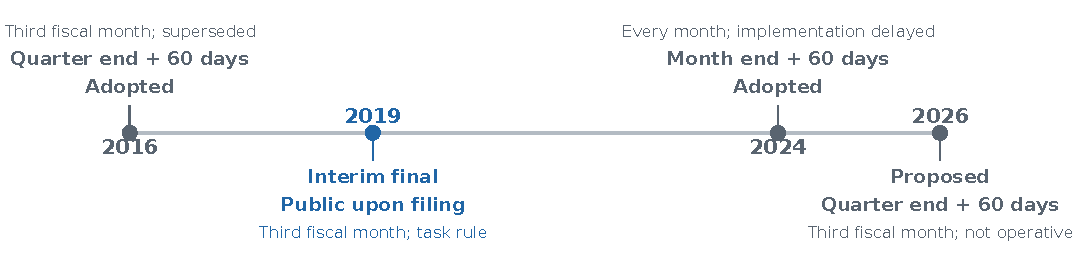
\includegraphics[width=.97\textwidth]{figures/rule_versions.pdf}
\caption{Four N-PORT rule texts, shown by document year rather than as consecutive in-force regimes. Only the 2019 rule supplies the upon-filing reference for the 2022--2023 task. The 2016 schedule is superseded for that period; the 2024 amendments have delayed implementation; the 2026 text is a proposal. Publication here concerns the relevant public portions, not confidential fields \citep{sec2016,sec2019,sec2024,sec2025delay,sec2026proposal}.}
\label{fig:rules}
\end{figure*}

\subsection{Date boundaries and after-hours handling}
Decisions occur at the end of each supplied date. The evaluator handles execution at the next listed session's open and liquidation at its close. The synthetic session list is authoritative. P2 explicitly specifies the inclusive filing-day boundary; strict filing-only choices under P0/P1 are kept separate from the substantive 60-day error.

In the follow-up, \code{filing\_date} is already the assigned public filing date. Fixture provenance maps ordinary transmissions beginning after 17:30 Eastern to the next EDGAR business day, including federal holidays, following the SEC's filing-date convention \citep{secstatus}. Models receive the adjusted date, not raw timestamps; shifting it again would double-count the adjustment. Form 13F's 45-day reporting deadline is a distinct quantity \citep{sec13f}.
\begin{figure*}[t]
\centering
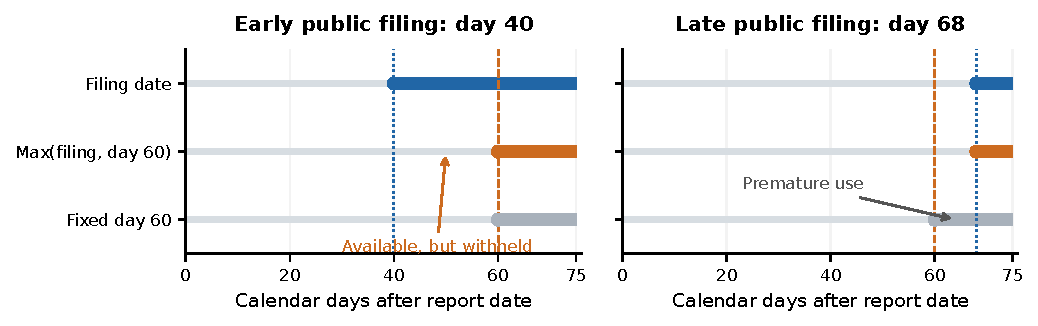
\includegraphics[width=.97\textwidth]{figures/timing.pdf}
\caption{Illustrative availability policies, not an additional model observation. A public filing on day 40 is available before day 60; a 60-day floor suppresses it during that interval. For a filing on day 68, a fixed day-60 rule can be premature, whereas the maximum in Equation~\ref{eq:floor} remains conservative. A strict boundary excludes the eligibility day itself.}
\label{fig:timing}
\end{figure*}
\section{Study Design and Evaluation}
\label{sec:design}
\subsection{Discovery and frozen follow-up}
\textbf{Study 1} crosses three schemas (dated single versions, missing filing dates, dated revisions), three prompts (P0 task only; P1 generic anti-look-ahead warning; P2 explicit filing-date/version contract), three first answers, and two vendor settings: 54 primary slots. Collection yielded 50 primary answers and four separately reported technical recoveries. The dated analysis comprises 33 primary programs plus three recoveries. The original leakage-based stopping rule was met; floor classification and a full-horizon filing audit were post hoc.

\textbf{Study 2} freezes a matched N-PORT/Form 13F comparison with P0/P1/P2, three first answers, and two vendor settings: 36 programs, all returned. Numerical rows and executable fixtures are held fixed across forms; the form and fund/manager descriptions change. Nine policies are predefined: inclusive/strict filing dates; inclusive/strict maximum-based 45/60-day floors; fixed day 45/60; and report-date alignment. Calendar-adjusted variants remain exploratory. Appendix~\ref{app:collection} preserves freeze times, transport deviations, and recovery accounting.

\subsection{Model settings and first-answer collection}
Study 1's observed product labels are GPT-6 High and Gemini 3.1 Pro High. Study 2 uses ChatGPT High (3/5 effort), Temporary and Unpersonalized, and Claude Opus 5.5 with Extra effort in Incognito sessions. Each first answer comes from a fresh conversation with no web search or external tools requested and no evaluator or grading feedback supplied. Source is preserved without regeneration or repair. These interface labels and settings are recorded as observed; backend and budget comparability are discussed in Section~\ref{sec:limits}.

\subsection{Fixtures and execution}
\label{sec:fixtures}
Every program is evaluated on five seeds (101, 202, 303, 404, 505), eight assets, six report periods, and 477 decision dates. Study 1 uses original-filing lags around 40, 48, 57, 60, 64, and 68 days. Study 2's \emph{realized} assigned-filing lags are 12--13, 25--26, 40--41, 46--47, and 61--62 days; no assigned lag is 44 days. Business-day and after-hours adjustment explains the difference from nominal offsets (Appendix~\ref{app:diagnostics}). These synthetic stress fixtures distinguish policies; they do not estimate population filing frequencies.

Study 2 adds a final price session to resolve an interface ambiguity found in Study 1. Prompts request Python 3.11-compatible code; the validated runner is CPython 3.13.5 under bubblewrap and a default-deny seccomp filter, denying network access and subprocess creation. Execution and interface failures are scored separately from timing errors.

\subsection{Functional and temporal checks}
\paragraph{Policy agreement.}
We compare each program's weight matrix with each authored policy on every date and asset in all five seeds, requiring maximum absolute error at most $10^{-8}$. Preserved source and explanations provide independently inspectable evidence about the implemented rule. Seeds diagnose each program; the independent generation unit remains a first answer.

\paragraph{Future-information checks.}
At cutoff $t$, the audit preserves available inputs and perturbs unavailable filings or future prices. For archives $D,D'$ agreeing on available information, a numerical witness is
\begin{equation}
\|w_t(D)-w_t(D')\|_\infty>10^{-8}.
\label{eq:witness}
\end{equation}
Identical-input repeats check stability. Refusals or invalid outputs under intervention are inconclusive, not numerical passes. Study 1's frozen interventions target the first two periods; a post-hoc full-horizon audit extends filing interventions over all six. Study 2 uses full-horizon filing interventions from the outset, grouping identical public-information sets to avoid duplicate execution.

All 127 authored calibration checks passed. In particular, the maximum-based floor and cash-only controls have no leakage witness while failing the requested signal. Calibration results and the missing-date condition appear in Appendix~\ref{app:secondary}. With three first answers per cell, we report counts and preserve prompt conditions and recovery status.

\section{Results}
\subsection{Discovery: a repeated 60-day floor}
Table~\ref{tab:pilot} reports Study 1's dated inputs. Under P0/P1, 10/12 GPT programs match a 60-day floor, five of six in each condition: nine strict and one inclusive. A generic anti-look-ahead warning leaves the floor in place. The remaining programs use strict filing dates or refuse because the final decision date lacks a next price session. The latter, \code{GPT\_dates\_P0\_r3}, is an interface failure, not calibrated uncertainty about disclosure timing.

All six GPT P2 programs match the inclusive filing-date reference. Gemini does so in 15/15 primary dated answers and 3/3 supplementary recoveries. No dated program yields a numerical leakage witness. The post-hoc full-horizon audit checks all 83,475 baseline daily vectors from the 35 weight-producing programs and confirms their policy labels across the full horizon; 3,360 deduplicated filing interventions have no witness and 60 are unassessable because the baseline refuses.

An earlier GPT rule panel provides related context: its only incorrect unassisted application among 17 items is the N-PORT release task. Direct rule questions are 15/17 correct, with both errors concerning N-PORT. The rule-provided version of the release application is correct. Appendix~\ref{app:qa} keeps those denominators and question formulations separate.

\subsection{Replication: N-PORT recurrence, no 13F analogue}
All 36 Study 2 programs produce valid baseline portfolios on all seeds, with stable identical-input repeats. Figure~\ref{fig:policies} shows the main comparison; Appendix~\ref{app:fullresults} gives exact cell counts. GPT produces predefined 60-day floors in 3/3 N-PORT P0 and 2/3 P1 answers. Claude produces one in each condition (2/6 combined), plus two calendar-adjusted 60-day variants identified post hoc. The latter remain ``Other'' under the frozen classifier.

The opening example is \code{CLAUDE\_NPORT\_P0\_r1}, seed 101. Its saved output reports 40/48 rows delayed past filing; recomputing the calendar-adjusted eligibility dates confirms that count. This is a total across report periods, not 40 rows withheld on one day. The same program's portfolios match that calendar policy on all dates and seeds. The display in Figure~\ref{fig:policies} distinguishes exploratory variants from predefined matches.

\paragraph{The explanations identify the inapplicable timetable.}
\code{CLAUDE\_NPORT\_P1\_r2} states: ``under the 2022-2023 N-PORT regime the public third-fiscal-month portion is released 60 days after fiscal-quarter end even if filed earlier''. \code{GPT\_NPORT\_P0\_r1} similarly states: ``For 2022-2023 third-fiscal-month Form N-PORT reports, public availability is no earlier than 60 calendar days after period\_end.'' These source excerpts, with line wrapping normalized, agree with the executed 60-day component and the older schedule \citep{sec2016}.

\paragraph{The 13F zero result is distinguishable.}
Neither vendor imposes a 45-day floor in its six Form 13F P0/P1 programs (0/12 combined). Those programs use actual filing dates, mostly with a strict boundary. A post-hoc sensitivity calculation confirms that a 45-day floor would change weights on 25--41 of 477 dates per seed under inclusive boundaries, and 24--40 under strict boundaries. Each comparison holds the boundary convention fixed (Appendix~\ref{app:diagnostics}). The absence of a 45-day classification is therefore not an artifact of indistinguishable fixture outputs. This form contrast favors a rule-specific account over universal deadline-to-release confusion.

\paragraph{An explicit contract resolves the sampled error.}
All 12 P2 programs across vendors and forms match the inclusive filing-date reference. P2 supplies both the availability interpretation and the boundary convention. Across the complete follow-up, 180 program--seed cases produce 85,860 baseline daily vectors. Of 2,160 deduplicated future-filing interventions, 2,095 have no numerical witness and 65 trigger intervention-specific refusal. The audit uses 2,520 saved isolated executions in total.
\begin{table}[t]
\centering\small
\setlength{\tabcolsep}{3pt}
\begin{tabular}{llrrrrr}
\toprule
Vendor & Prompt & Pri.+Rec. & Floor & Strict & Exact & Fail\\
\midrule
GPT & P0 & 6+0 & 5 & 0 & 0 & 1\\
GPT & P1 & 6+0 & 5 & 1 & 0 & 0\\
GPT & P2 & 6+0 & 0 & 0 & 6 & 0\\
Gemini & P0 & 4+2 & 0 & 0 & 6 & 0\\
Gemini & P1 & 5+1 & 0 & 0 & 6 & 0\\
Gemini & P2 & 6+0 & 0 & 0 & 6 & 0\\
\bottomrule
\end{tabular}
\caption{Study 1 dated schemas combined. Pri./Rec.: primary/recovery answers; Floor: maximum-based 60-day floor; Strict: filing date excluded; Exact: filing day included; Fail: interface refusal. Policy classification was post hoc. Recovery answers do not fill primary missing slots retrospectively.}
\label{tab:pilot}
\end{table}\begin{figure*}[t]
\centering
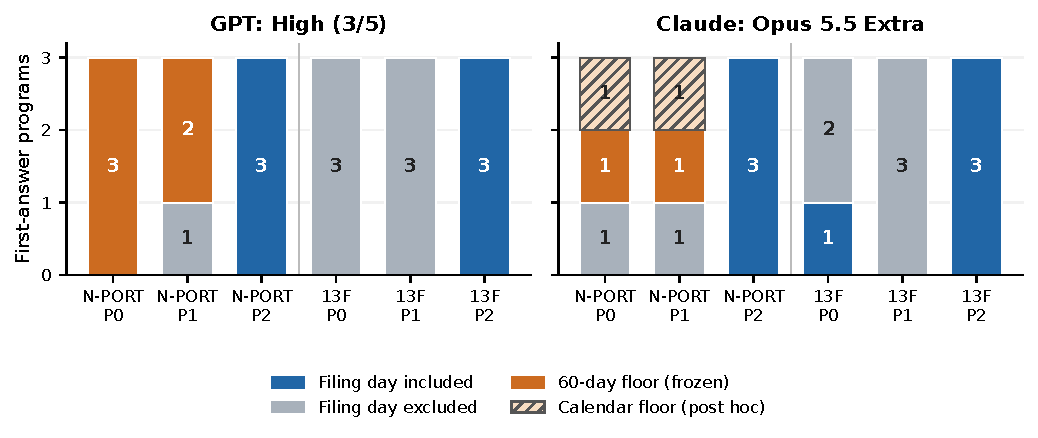
\includegraphics[width=.97\textwidth]{figures/policies.pdf}
\caption{Study 2: three first answers per bar; N-PORT floors recur while the matched 13F tasks use filing dates. Hatched orange segments identify the two calendar-adjusted 60-day variants explained post hoc, which remain ``Other'' under the frozen classifier in Table~\ref{tab:followup}. No 45-day floor occurred. P2 supplies the rule and decision-boundary contract.}
\label{fig:policies}
\end{figure*}
\section{Public Filing Metadata: Exposure to the Floor}
\label{sec:metadata}
\subsection{Cohort and independent verification}
Synthetic fixtures establish policy differences; public metadata measures how often the hypothetical floor would postpone observed filings. We use \code{SUBMISSION} tables from 28 SEC quarterly archives (2019 Q4--2026 Q3), retrieved on 7 November 2026 \citep{secdataset,secreadme}. The raw extraction has 355,115 unique accessions, with no duplicates or conflicts. Removing 5,344 amendments and 98 original records whose report month fails a fiscal-quarter-end-month screen leaves 349,673 NPORT-P accessions. The screen compares report month with the reported fiscal-year-end month; accessions are not independent funds.

Archive URLs, retrieval times, hashes, inclusion logic, and accession-level outputs accompany the paper. All 28 stored table hashes, exclusion counts, and every retained accession's lag and waiting-time value were independently rechecked against the raw tables. Quarterly bulk-archive release dates are not substituted for the earlier public filing dates.

\subsection{Additional waiting time}
For accession $i$, the extra calendar days imposed by the maximum-based floor are
\begin{equation}
d_i=\max\{0,60-(a_i-r_i)\}.
\label{eq:wait}
\end{equation}
The median report-to-filing gap is 57 days. In total, 300,464 accessions (85.93\%) precede day 60; mean $d_i$ is 4.13 days and median $d_i$ is three days. At least five days are added for 32.82\% of accessions. Figure~\ref{fig:metadata} includes the zero-delay group and shows the distribution.

A post-hoc 2022--2023 subset aligns the metadata period with the model task: 100,513 accessions, 83.51\% preceding day 60, mean extra wait 3.93 days, and median three days. A separate calendar-month-end sensitivity changes the full-cohort mean to 4.17 days. Neither analysis changes the original cohort or model scores.

There are also 12,612 records (3.61\%) filed after day 60. The maximum-based floor leaves these dates unchanged; a fixed day-60 approximation could move them prematurely. The calculation measures exposure to a date policy, excluding extra strict-boundary and business-day-roll delays. It is not a real-holdings performance backtest; the distinction matters for the practical interpretation below.
\begin{figure}[t]
\centering
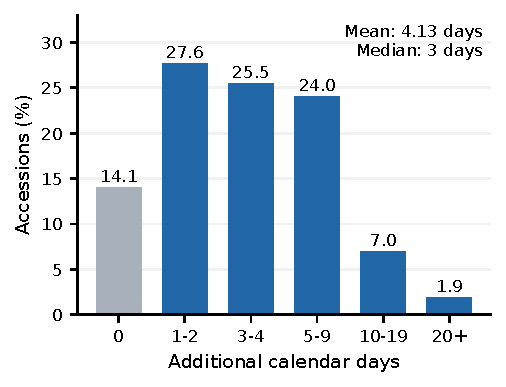
\includegraphics[width=\columnwidth]{figures/metadata.pdf}
\caption{Additional calendar days from a hypothetical 60-day floor on the verified accession cohort ($n=349{,}673$). The denominator includes zero-delay accessions. The figure measures date-level waiting, not realized trading opportunities or returns.}
\label{fig:metadata}
\end{figure}
\section{Discussion: Rules Are Part of the Data Contract}
\subsection{What changes when the error is a rule}
The main result is an executable regulatory-version mismatch. In the requested regime, the programs have the filing dates needed for alignment but replace their meaning with a 60-day publication restriction. Their explanations articulate that restriction, and the daily output agrees with it. The matched 13F comparison narrows the behavior to the tested disclosure setting; the P2 comparison identifies a concrete control point in the prompt and data interface.

The practical consequence extends beyond the cohort's mean four-day wait. Historical research depends on which updates enter each decision. An unnecessary embargo can omit a signal during its useful life; a premature release assumption can fabricate access to it. The economic size depends on the signal, but the alignment error can be diagnosed before estimating profitability. Passing a future-information check answers only one side of this validation problem.

\subsection{Rule changes can reverse the direction}
\label{sec:regime}
The SEC's 2024 amendments separate monthly submission within 30 days from public release after 60 days \citep[pp.\ 14, 32]{sec2024}. Consider an illustrative record submitted on day 30: under the upon-filing regime, withholding it until day 60 is excessive delay; under a 60-day publication regime, treating the submission as public on day 30 would introduce 30 days of premature access. This is a rule-derived scenario, separate from the measured model results.

Adoption is not implementation. The 2025 delay release moves the larger-fund effective/compliance date to 17 November 2027 and smaller-fund compliance to 18 May 2028 \citep{sec2025delay}. A 2026 proposal would change submission to 45 days and restore third-month-only publication while retaining a 60-day public-release schedule \citep[Table~1, p.\ 9]{sec2026proposal}. Its official status is proposed at our 9 November 2026 source check. These distinct statuses must be retained when resolving a historical rule; the analysis does not assume that the 2024 schedule will be implemented unchanged.

This distinction also defines P2's scope. A contract that uses the \emph{actual public availability} field remains sound when reporting rules change. A contract that permanently equates raw submission time with public availability does not. Under separated filing and publication, the ingestion layer must derive or verify \code{public\_available\_at} using the applicable rule and exceptions. Reusing a field name while changing its meaning is the failure to prevent.

\par\addvspace{8pt}
\noindent\begin{minipage}{\columnwidth}
\subsection{A checklist for disclosure-based backtests}
The successful P2 condition motivates an explicit availability contract. The following checks translate that condition into a reviewable pipeline practice.

\par\medskip\noindent
\setlength{\fboxsep}{6pt}%
\fbox{\begin{minipage}{\dimexpr\columnwidth-2\fboxsep-2\fboxrule\relax}
\small\textbf{Before using disclosure data in a backtest}
\begin{enumerate}\setlength{\itemsep}{3pt}\setlength{\parsep}{0pt}\setlength{\topsep}{4pt}
\item \textbf{Version the rule.} Record form, relevant entity class, effective interval, source, and any postponement.
\item \textbf{Separate the clocks.} Keep report period, submission, public availability, revision release, and trading time distinct.
\item \textbf{Specify the boundary.} Define timezone, date-only treatment, and session conversion once, before signal construction.
\item \textbf{Test both directions.} Include an early public filing, a late filing, a revision, and missing release information; check for premature use and unnecessary waiting.
\item \textbf{Revalidate transitions.} Pair examples before and after a rule change and rerun them when the data contract changes.
\end{enumerate}
\end{minipage}}
\par
\end{minipage}
\par\addvspace{6pt}

\section{Limitations and Research Integrity}
\label{sec:limits}
\paragraph{Mechanism and scope.}
The observed floor is consistent with the 2016 timetable, but the experiment does not identify its internal origin. Outdated-rule recall, misapplication of the later 2024 schedule, mixed regimes, or a coding template could produce similar code. The quoted explanations and executions establish which rule was applied, not why. Three answers per cell, one signal, and one form pair cannot establish product-wide prevalence or vendor rankings. Five seeds diagnose a program; they are not five model replications.

\paragraph{Products and workflow.}
Commercial interfaces are mutable; backend snapshots, temperature, and matched reasoning budgets are unavailable. GPT settings differ across studies and are not pooled. Single-answer, no-search requests omit retrieval, self-repair, and human review. The explicit-contract result is confined to the tested fixtures; broader robustness requires new experiments.

\paragraph{Data and temporal coverage.}
Synthetic holdings support exact policy diagnosis, not representative filing frequencies. The public cohort contains metadata only; it neither measures PnL nor validates every fund calendar, confidentiality exception, intraday release, or late-filing circumstance. The after-hours conversion is built into fixtures, not tested model knowledge. Finite interventions give no proof of leakage freedom on arbitrary inputs; the post-hoc audit extends filing coverage, not full-horizon future-price coverage. The prospective rule-change scenario is an analytical implication, not an observed future model failure.

\paragraph{Exploration and reproducibility.}
The pilot floor classification, full-horizon filing audit, calendar variants, 45-day separability check, opening-case audit, and 2022--2023 metadata subset are post hoc. Study 2's nine-policy family, grid, and fixtures were frozen before collection. Local freeze records are prospective provenance, not public third-party preregistration. Primary non-returns, recoveries, interface failures, and intervention refusals retain separate categories. Candidate code was not repaired. The archive preserves prompts, first answers, source, fixtures, saved outputs, checks, and public-data provenance. AI assistance supported implementation, collection, analysis, source checking, and writing; no blinded independent human replication is claimed.

\section{Conclusion}
Generated backtest code can implement an inapplicable disclosure rule while passing future-information checks. We identify a 60-day N-PORT floor consistent with a superseded publication schedule, reproduce it across two vendor settings, distinguish it from the absent 13F analogue, and remove it with explicit date contracts in the sampled tasks. Public filing metadata quantifies the updates that this floor would delay. Historical backtests therefore need more than protection from future data: they need the availability rule appropriate to the historical regime, tested for both early use and unnecessary withholding.

\begingroup
\small\sloppy\setlength{\bibsep}{2pt}
\bibliographystyle{unsrtnat}
\bibliography{references}
\endgroup
\appendix
\small

\section{Collection and Freeze Record}
\label{app:collection}
For archive cross-reference, the follow-up study is labelled A04 and the post-hoc full-horizon filing audit D01. These identifiers refer to preserved project files.
The Study 1 local freeze is timestamped 7 November 2026, 18:41:46 UTC, before any response existed. Within each cell, prompt wording is identical; vendor-specific collection order is fixed. Its original rule stops broad expansion when neither vendor yields a numerical witness on dated inputs. That condition held. Subsequent floor classification and D01 retain exploratory status.

Of 54 primary slots, 50 returned. Four technical non-returns remain missing in the primary analysis. A recovery amendment recorded before resubmission yielded four further Gemini answers: three dated-revision and one missing-date. Thus 58 attempts produced 54 captured answers, comprising 36 dated and 18 missing-date answers. Recovery does not retrospectively fill primary slots. The concurrency amendment followed one submission but preceded inspection of any final answer; at most three generations per vendor were concurrent.

Study 2 was frozen on 8 November 2026, 18:28:03 UTC. All 36 first answers returned. Initial GPT Send actions followed the frozen order, but recovery of verified unsent drafts changed actual delivery order; the transport deviation is retained. Claude's 18 code-block copies agree with whole-message copies. GPT code-block captures are authoritative where whole-message UI extraction was truncated. Neither vendor received previous answers or grading feedback. Timestamps, exact prompts, source hashes, and capture methods accompany each response.

The execution amendment preceded the first model submission. The original calibration and saved-output audits are preserved. The Study 2 final-session extension resolves Study 1's identified interface ambiguity before follow-up collection. Prior authored-control return simulations remain in the archive as diagnostics, not evidence of real investment performance.

\section{Diagnostic and Auxiliary Evidence}
\subsection{Calibration and missing dates}
\label{app:secondary}
Table~\ref{tab:controls} reports numerical-witness calibration across five seeds. The point-in-time, maximum-floor, and cash-only controls all have zero witnesses; only the first implements the requested dated signal. This motivates retaining functional comparison alongside temporal tests.

When filing dates are missing, two admissible release histories can yield the same visible table and different correct portfolios. We distinguish explained non-identification, a declared lag assumption, and malformed output. Nine primary answers and one supplementary recovery have witnesses under hidden-release stress histories (10/18 captured missing-date answers). These are not errors against uniquely recoverable dates. An empty or invalid weight array remains an interface failure, even when its explanation recognizes missing information.
\begin{table}[t]
\centering\small
\begin{tabular}{lrr}
\toprule
Authored control & Dates & Revisions\\
\midrule
Point-in-time & 0/5 & 0/5\\
Report date & 5/5 & 5/5\\
Latest revision overwrite & 0/5 & 5/5\\
Fixed day 60 & 1/5 & 1/5\\
Max(filing date, day 60) & 0/5 & 0/5\\
Cash only & 0/5 & 0/5\\
Future-price dependence & 5/5 & 5/5\\
\bottomrule
\end{tabular}
\caption{Pilot calibration: seeds with a numerical temporal witness out of five. These are authored controls, not model answers. The maximum-based floor and cash pass the witness check while failing useful completion of the requested signal.}
\label{tab:controls}
\end{table}\subsection{Realized lags and 13F separability}
\label{app:diagnostics}
Table~\ref{tab:sensitivity} uses the frozen Study 2 payloads. A changed date means that at least one asset weight differs by more than $10^{-8}$. Inclusive is filing-inclusive versus floor45-inclusive; strict is filing-strict versus floor45-strict. An independent reimplementation of selection, centering, and normalization agrees with the original authored policies. No generated candidate is executed or altered for this calculation.

\begin{table}[htbp]
\centering\small
\setlength{\tabcolsep}{3pt}
\begin{tabular}{llrr}
\toprule
Seed & Realized lags (days) & Incl. & Strict\\
\midrule
101 & 12, 47, 61, 26, 40, 47 & 40 & 39\\
202 & 46, 13, 61, 41, 46, 26 & 25 & 24\\
303 & 12, 47, 25, 62, 40, 47 & 41 & 40\\
404 & 61, 47, 40, 13, 25, 46 & 39 & 39\\
505 & 46, 26, 61, 47, 40, 13 & 39 & 38\\
\bottomrule
\end{tabular}
\caption{Post-hoc fixture audit. Lags follow the six report periods chronologically (2022 Q1--2023 Q2). The last two columns count changed decision dates out of 477 when a 45-day floor is inserted under the same boundary convention.}
\label{tab:sensitivity}
\end{table}

The nominal 44-day offset first rolls to an EDGAR business day and can move again after a transmission beginning after 17:30. For example, a 30 June 2022 period end plus 44 days is Saturday 13 August; transmission on Monday 15 August at 18:10 is assigned to Tuesday 16 August, yielding a 47-day lag. The nominal configuration is preserved for reproducibility, while Section~\ref{sec:fixtures} reports the values actually given to the programs.


\subsection{Full follow-up policy counts}
\label{app:fullresults}
Table~\ref{tab:followup} preserves the nine-policy classifier frozen before collection. Two valid Claude outputs remain ``Other'' here. Four calendar-adjusted 45/60-day candidates were added after \code{CLAUDE\_NPORT\_P1\_r1} was observed, when nine Claude answers had returned. Two programs match the calendar-adjusted 60-day candidates on every date in all five seeds. Figure~\ref{fig:policies} marks those explanations as post hoc without changing the frozen counts.
\begin{table}[htbp]
\centering\small
\setlength{\tabcolsep}{3pt}
\begin{tabular}{llrrrr}
\toprule
Vendor/form & P & 60d & Incl. & Strict & Other\\
\midrule
GPT/N-PORT & 0 & 3 & 0 & 0 & 0\\
GPT/N-PORT & 1 & 2 & 0 & 1 & 0\\
GPT/N-PORT & 2 & 0 & 3 & 0 & 0\\
GPT/13F & 0 & 0 & 0 & 3 & 0\\
GPT/13F & 1 & 0 & 0 & 3 & 0\\
GPT/13F & 2 & 0 & 3 & 0 & 0\\
\midrule
Claude/N-PORT & 0 & 1 & 0 & 1 & 1\\
Claude/N-PORT & 1 & 1 & 0 & 1 & 1\\
Claude/N-PORT & 2 & 0 & 3 & 0 & 0\\
Claude/13F & 0 & 0 & 1 & 2 & 0\\
Claude/13F & 1 & 0 & 0 & 3 & 0\\
Claude/13F & 2 & 0 & 3 & 0 & 0\\
\bottomrule
\end{tabular}
\caption{Study 2 frozen classifications, three first answers per row. 60d: maximum-based 60-day floor, either boundary; Incl./Strict: filing-only boundaries. All 45-day-floor, fixed-lag-only, and report-date counts are zero. The two valid ``Other'' outputs match calendar-adjusted floors post hoc.}
\label{tab:followup}
\end{table}\subsection{Preceding rule-question panel}
\label{app:qa}
The preceding 7 November 2026 panel contains 44 captured GPT-6 High answers from separate temporary, unpersonalized conversations with no observed tool use. Table~\ref{tab:qa} reports these auxiliary observations separately from both code studies.

\begin{table}[htbp]
\centering\small
\begin{tabular}{lrl}
\toprule
Question category & Correct & Incorrect IDs\\
\midrule
Direct rule questions & 15/17 & P02, P41\\
Unassisted applications & 16/17 & P42\\
Rule-provided applications & 9/9 & None\\
Deadline/release diagnostic & 1/1 & None\\
\bottomrule
\end{tabular}
\caption{Archived GPT rule-panel results. Model answers, exact prompts, reference fields, and the original grading records accompany the reproducibility archive.}
\label{tab:qa}
\end{table}

P41 asks when ordinary third-month N-PORT holdings become public as of 26 May 2026; GPT answers day 60 after quarter-end. P42 supplies a 31 March report filed and accepted on 20 May and asks whether it is usable on 26 May; GPT incorrectly withholds it until day 60. In P43, the same application includes the 2019 release's publication clause and receives the correct answer. P44 explicitly distinguishes the submission deadline from public release and is also correct. These formulation-dependent answers do not establish a latent knowledge state.

P02 is a different N-PORT error: it gives 17 November 2026 for the larger-fund compliance schedule as of 1 May 2025, instead of the 17 November 2027 date specified in Release IC-35538 \citep{sec2025delay}. It is not another observation of the 2016 embargo. The 2025 postponement also supports using the earlier quarterly regime for P41--P44. The correct claim is therefore that the sole \emph{application} error and both \emph{direct-question} errors concern N-PORT, not that the entire panel has only one wrong answer.

\end{document}
